%%%%%%%%%%%%%%%%%%%%%%%%%%%%%%%%%%%%%%%%%%%%%%%%%%%%%%%%%%%%%%%%%%%%%%%%%%%%%%%%
%2345678901234567890123456789012345678901234567890123456789012345678901234567890
%        1         2         3         4         5         6         7         8

\documentclass[letterpaper, 10 pt, conference]{ieeeconf}  % Comment this line out if you need a4paper

%\documentclass[a4paper, 10pt, conference]{ieeeconf}      % Use this line for a4 paper

% \IEEEoverridecommandlockouts                              % This command is only needed if
                                                          % you want to use the \thanks command

\overrideIEEEmargins                                      % Needed to meet printer requirements.

%In case you encounter the following error:
%Error 1010 The PDF file may be corrupt (unable to open PDF file) OR
%Error 1000 An error occurred while parsing a contents stream. Unable to analyze the PDF file.
%This is a known problem with pdfLaTeX conversion filter. The file cannot be opened with acrobat reader
%Please use one of the alternatives below to circumvent this error by uncommenting one or the other
%\pdfobjcompresslevel=0
%\pdfminorversion=4

% See the \addtolength command later in the file to balance the column lengths
% on the last page of the document

% The following packages can be found on http:\\www.ctan.org
\usepackage{graphicx} % for pdf, bitmapped graphics files
%\usepackage{epsfig} % for postscript graphics files
%\usepackage{mathptmx} % assumes new font selection scheme installed
%\usepackage{times} % assumes new font selection scheme installed
\usepackage{amsmath} % assumes amsmath package installed
\usepackage{amssymb}  % assumes amsmath package installed
%\usepackage{dsfont}
\usepackage{algorithm}
\usepackage{algorithmic}
\usepackage{commath}

\usepackage{xcolor}
\newcommand{\todo}[1]{{\color{blue}[TODO: #1]}}
\newcommand{\response}[1]{{\color{green}[RESPONSE: #1]}}

\DeclareMathOperator*{\argmax}{arg\,max}
\DeclareMathOperator*{\argmin}{arg\,min}

\title{\LARGE \bf
Optimal Multi-Agent Coverage and Flight Time with Genetic Path Planning
}

\author{Jacob M. Olson$^{1}$, Craig C. Bidstrup, Brady K Anderson, Alan R. Parkinson$^{2}$% <-this % stops a space
%\thanks{This research was supported through the Center for Unmanned Aircraft Systems (C-UAS), a National Science Foundation-sponsored industry/university cooperative research center (I/UCRC) under NSF Award No. IIP-1650547 along with significant contributions from C-UAS industry members.}% <-this % stops a space
\thanks{$^{1}$The corresponding author can be contacted at
        {\tt\small jacobmo at byu.edu}.}%
\thanks{$^{2}$All authors are with the Department of Mechanical Engineering or Electrical and Computer Engineering,
        Brigham Young University, Provo, UT, 84602, USA.}%
%\thanks{$^{3}$C. Peterson is with the Faculty of Electrical and Computer Engineering,
%		Brigham Young University, Provo, UT, 84602, USA.
%        {\tt\small cammy.peterson at byu.edu}}%
%\thanks{$^{4}$R. W. Beard is with the Faculty of Electrical and Computer Engineering,
%		Brigham Young University, Provo, UT, 84602, USA.
%        {\tt\small beard at byu.edu}}%
}

\begin{document}

\maketitle
\thispagestyle{empty}
\pagestyle{empty}


%%%%%%%%%%%%%%%%%%%%%%%%%%%%%%%%%%%%%%%%%%%%%%%%%%%%%%%%%%%%%%%%%%%%%%%%%%%%%%%%
\begin{abstract}

When generating 3D maps with unmanned aerial vehicles (UAVs), it is important for the mapping algorithm to have good coverage of the environment. It is also important, especially when planning paths for multiple agents to have loop closures along each flight path and with other agents. Because multirotor UAVs are limited in flight time, the flight paths must be limited in length. Generating a good flight path to map a new environment can be difficult and tedious because of the free-form nature of a flight path. To solve this problem, we propose using a genetic algorithm designed to maximize total area coverage while minimizing flight time and enforcing sufficient loop closures. The natural ability of genetic algorithms to rapidly explore a design space is advantageous when solving complex free-form problems like path planning.

\end{abstract}


%%%%%%%%%%%%%%%%%%%%%%%%%%%%%%%%%%%%%%%%%%%%%%%%%%%%%%%%%%%%%%%%%%%%%%%%%%%%%%%%
\section{INTRODUCTION}

%Talk about lit review and what we will be contributing to the space

%add multi agent to this
Autonomously generating an internal 3D map of a building requires intelligent control of the mapping vehicle. This ranges from manually planning a flight path with simple obstacle avoidance to full stack exploration and path planning algorithms.

Generating a flight path is a nontrivial task, especially when multiple objectives are considered. For example, the algorithm may want to maximize observed coverage of the space while minimizing flight time. This becomes tedious with each new space and more difficult as the complexity of the space increases with more rooms and inter-connecting hallways. When planning paths to achieve good coverage of the area rather than obstacle avoidance or traversability, it becomes much more complex. To plan effective flight paths in more complex flight spaces, using algorithms to plan the paths becomes a necessity.

When generating paths for the purpose of building a 3D map of the environment in a GPS-denied area such as indoors, enforcing loop closures becomes critical. Loop closures both between paths of different agents and between different segments of the same path are critical to successfully generate a usable map. Loop closures between different segments of the same path significantly reduce drift that occurs in visual odometry algorithms necessary for navigation and estimation with UAVs. Loop closures between paths of different agents ensures that the individual maps of each agent will combine into a single map.

There are several different approaches to coverage path planning that have been explored over recent years. These approaches range from 2D coverage where the robot must pass over all points in its known environment, common for uses such as cleaning robots or mine searching \cite{Choset2001} to using coverage planning to generate 3D maps of outdoor terrain using viewpoint information from the robot's camera \cite{Bircher2016}. These approaches differ from the coverage planning desired for generating 3D maps of indoor environments with multiple UAVs in that they do not enforce loop closures in the generated paths.

The complexity of the design space renders many simple optimization routines improper for this problem. Further, by the structure of the problem, derivatives are not available for each design variable. Thus, a derivative-free approach is required. We chose to use a genetic algorithm because they are well suited to this type of problem. As outlined by Gen et al. \cite{Gen2000}, genetic algorithms are a powerful tool for solving complex, multi-objective optimization problems such as this. Genetic algorithms have been used in coverage path planning before, Yakoubi et al. details an approach to 2D coverage planning of a cleaning robot using a multi-objective genetic algorithm \cite{Yakoubi2016} and Hameed discussed using them for 3D terrain \cite{Hameed2014}. Similarly to \cite{Choset2001}, and \cite{Bircher2016}, these approaches to not enforce loop closures and the objective is to visit all areas on the ground. Since the goal of this optimization is to get a path that when flown will generate a high fidelity 3D map of an indoor area, viewing all of the walls and obstacles is more important than visiting all areas on the ground. The genetic algorithm proposed in this paper takes these differences into consideration.

We first discretized and simplified the model as much as possible to shrink the design space before applying a genetic algorithm. We found our genetic algorithm was able to effectively plan single agent and multi-agent paths in an arbitrary environment and satisfy the constraints of the problem.

The remainder of the paper is organized as follows: Section \ref{setup} describes the method for simplifying the design space to create a reasonable problem for the genetic algorithm to solve. Section \ref{approach} describes the approach and architecture used to generate optimal paths for a single UAV, then the method is extended to multi-agent path planning.
Results showing and evaluating the generated paths are presented in Section \ref{results}. Finally, conclusions are presented in Section \ref{conclusions}.

%%%%%%%%%%%%%%%%%%%%%%%%%%%%%%%%%%%%%%%%%%%%%%%%%%%%%%%%%%%%%%%%%%%%%%%%%%%%%%%%
\section{OPTIMIZATION SETUP}\label{setup}

Modeling a problem for optimization requires a balance between fidelity and tractability. Model accuracy is especially important because any inaccuracies in the model can lead to solutions that are not truly optimal in the physical system. However, if the design space is too large, or ill formed, optimization algorithms can fail to converge. This is especially problematic when derivatives are not available, or there are multiple local optima.

\subsection{Problem Statement}


The goal of our optimization is to generate paths through a simple floor plan with the intent of building a 3D map using a UAV and an RGB-D (color and depth) camera. We start with a simple 2D floor plan of the area of interest and a known scale of the map. Then, with as little human interaction as possible, generate a flight path for the UAV to map the building, maximizing coverage while minimizing flight time so that the path is feasible with real hardware. We do this first with a single agent, then extend it to work for several agents collaborating to build a single map.

\subsection{Discretization}

The open-ended nature of path planning can make optimization difficult. To simplify the design space we discretize it as much as possible.

\subsubsection{Map Generation}

The first step to discretizing the design space is to simplify the 2D floor plan. The only part of discretization that must be done manually is segmenting explorable areas and occluded (inaccessible or uninteresting) areas on the 2D map. Fig. \ref{fig:map_gen} illustrates how this segmentation works. The white space represents explorable areas and black space represents occluded areas.

\begin{figure}
\centering
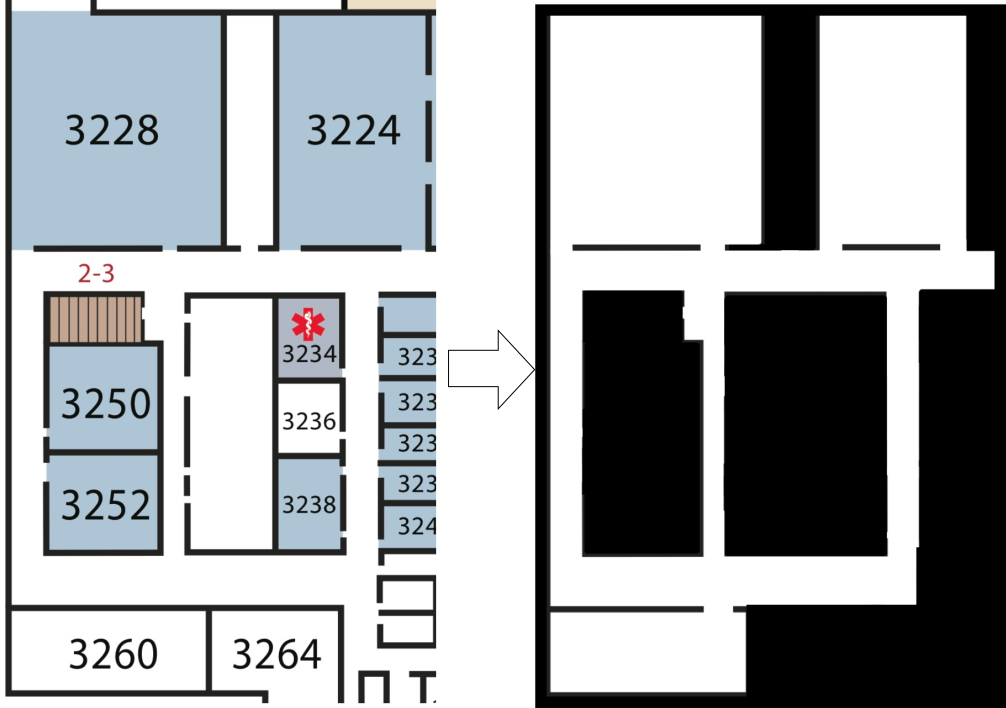
\includegraphics[width=0.8\linewidth]{figures/map_bw.png}
\caption{The initial 2D floor map of the area of interest and the segmented floor map reflecting explorable and occluded spaces.}
\label{fig:map_gen}
\end{figure}

Once this map is segmented, it is scaled to represent the minimum resolution desired in the optimization. This parameter is tunable to balance run time and fidelity. Once the map is properly scaled, we begin generating waypoints.

\subsubsection{Waypoints}

To further discretize and simplify the design space of the optimization, we place waypoints on the map and constrain the flight path to only fly through these waypoints. First, a grid is overlaid onto the map with a resolution of one half the width of the narrowest accessible hallway. This ensures that there are waypoints in every hallway and room to make the space fully traversable. Next, all waypoints overlapping occluded space are removed.

After removing occluded waypoints, the remaining waypoints are further pruned and adjusted to better cover the space. To remove waypoints that would cause the UAV to collide with obstacles, we generate a safety buffer around all occluded space greater than half the width of the UAV. Any waypoint that falls within this safety buffer is nudged away from the wall. The waypoints are then pruned to remove redundancy. The distance between adjacent waypoints is checked and any that are closer than the initial grid resolution are replaced with a single waypoint at the centroid of the cluster. This prevents over-crowding of waypoints in hallways and corners to make it simpler to generate flight paths in these areas. Fig. \ref{fig:waypoints} shows an example of this waypoint pruning process. Point A shows two waypoints being merged while Point B shows three. We chose to do this simplified discretization approach rather than computing Voronoi Graphs of the map as done by Sipahioglu et al. \cite{Sipahioglu2010} which tend to collapse rooms down into very few waypoints. We wanted to allow more open-ended exploration in open areas such as large rooms.

\begin{figure}
\centering
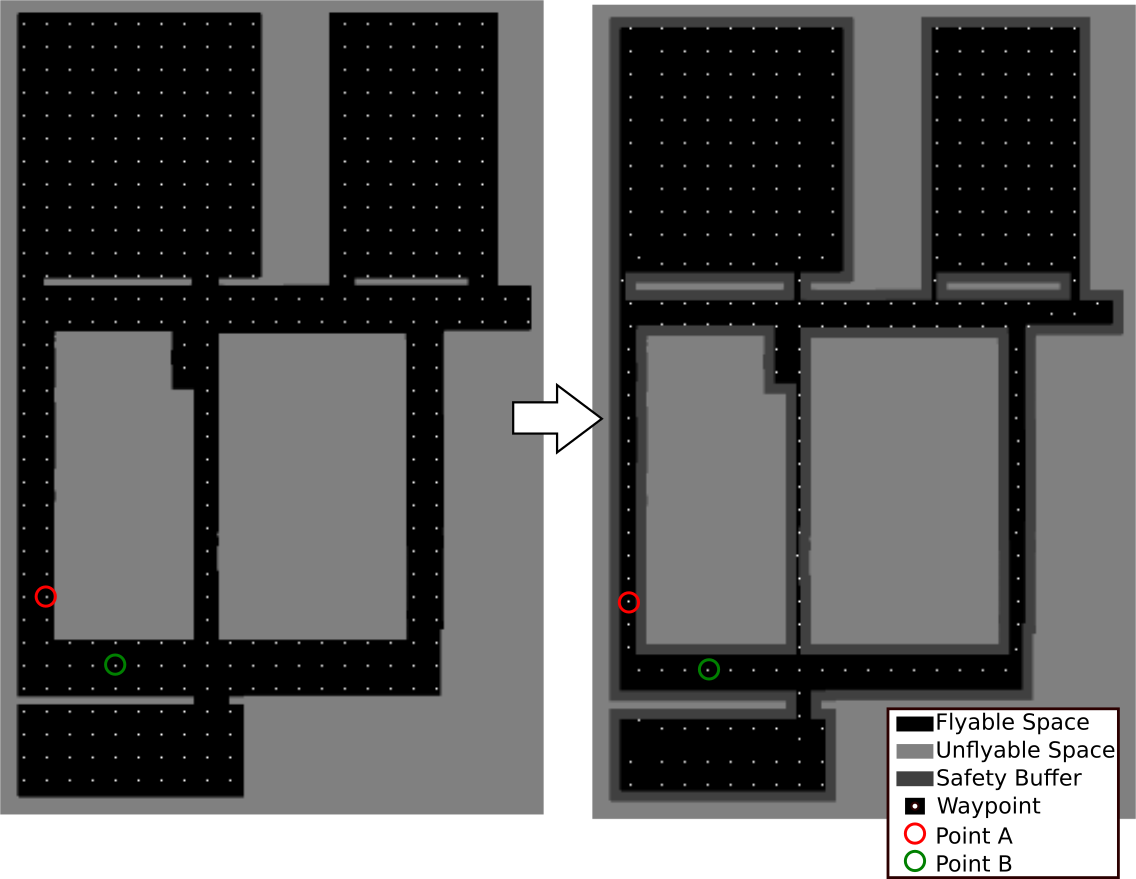
\includegraphics[width=0.8\linewidth]{figures/waypoint2.png}
\caption{The initial waypoint grid with only occluded waypoints removed (left) and the modified waypoint grid after applying the safety buffer and anti-crowding (right).}
\todo{make this figure more readable}
\label{fig:waypoints}
\end{figure}

\subsection{Objective Functions}

We split the optimization into two competing objectives. First, to maximize coverage of the given map, and second, to minimize flight time.

\subsubsection{Maximize Coverage}

The first objective is to maximize coverage of the environment.  To simplify the problem, we assume the UAV only flies forward. We use the camera's minimum and maximum viewable depths ($d_{min}$ and $d_{max}$) and horizontal field of view ($\theta_{fov}$) to construct the camera viewable area. Then at each camera pose, we subtract all explorable area occluded by obstacles from the viewable area by dividing the viewable area into $m$ sections and setting the distance of each section $d_{view,i}$ to

\begin{align}
  d_{view,i} &= max(min(d_{max}, min(d_{obs,i})),d_{min}) \\
  i &= 0...m \nonumber
\end{align}

where $d_{obs,i}$ is an array composed of the distances to all obstacles in section $i$. As $m$ increases, the coverage calculation becomes more accurate, but also more more computationally costly. An example of how the coverage is evaluated is shown in Fig. \ref{fig:coverage_sections}.

\begin{figure}
\centering
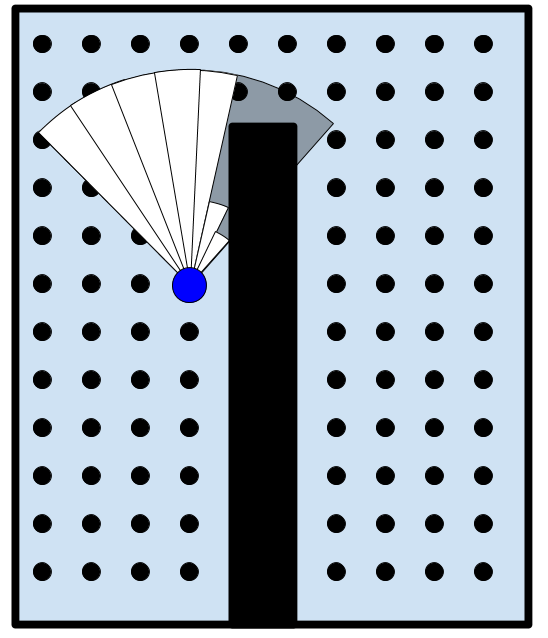
\includegraphics[width=0.5\linewidth]{figures/coverage_sections.png}
\caption{An example of how the coverage would be evaluated at a single waypoint with $m$=7. The blue dot is the agent at a waypoint, the white area is what would be counted as viewed and the grey area represents the maximum viewable area.}
\label{fig:coverage_sections}
\end{figure}

We then set the modified viewable area as explored at a waypoint. After repeating this process for every waypoint in the path, we calculate the percent of the explorable space in the map that is seen in that path. Mapping and visual odometry algorithms work better when the color and depth information from the camera is feature rich. Because of this, flying near walls is more beneficial than flying in open space like the middle of large rooms. To capture this, we compute a second coverage value which is the percent of safety buffer (computed when placing waypoints) seen by the path. We then preform an alpha blend (shown in equation \ref{eq:coverage}) on the two coverage types to get a single value that is used as the first objective value.

\begin{equation}\label{eq:coverage}%\nonumber
    \mathcal{C} = \alpha_{cov} \mathcal{C}_{open} + \left(1-\alpha_{cov})\right. \mathcal{C}_{walls}
\end{equation}

Where $\mathcal{C}$ is the value used for the coverage constraint, $\mathcal{C}_{open}$ is the coverage of the open explorable space, $\mathcal{C}_{walls}$ is the coverage of the safety buffer, and $\alpha_{cov}$ is a tunable parameter to weight the importance of walls vs. empty space in the coverage calculation. See Fig. \ref{fig:coverage} for an example path and corresponding coverage from this step.

\begin{figure}
\centering
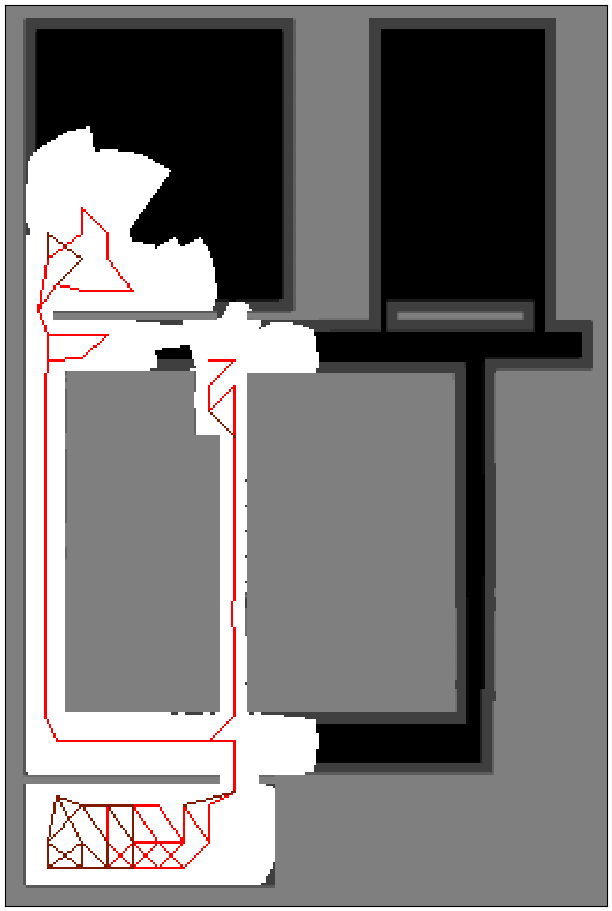
\includegraphics[width=0.8\linewidth]{figures/coverage_map3.png}
\caption{An example path and its corresponding coverage. The red line is the path flown, light grey represents obstacles, white represents explored area, black represents unexplored open space, and dark grey represents unexplored walls}
\label{fig:coverage}
\end{figure}

\subsubsection{Minimize Flight Time}

The second objective function minimizes flight time. To achieve this, we assume a constant velocity flight and compute the total distance flown in each path. To avoid meandering too much and incentivize flying straight lines, we also added a turning cost proportional to the change in heading angle between waypoints.

\begin{equation}%\nonumber
    \text{flight time} = \sum_{i=0}^{l} (d_{w,i} + \rho\abs{\Delta \psi_i})
\end{equation}

Where $l$ is the total number of waypoints in a given path, $d_{w,i}$ is the distance between the current waypoint and the next waypoint, $\rho$ is a tunable parameter to weight the cost of turning, and $\Delta \psi_i$ is the difference in heading angle between the current and next waypoint. This favors paths with fewer waypoints and less turning.

\subsection{Traversable Graph}

To save computation when generating or modifying paths, we pre-compute the traversability graph. The UAV is allowed to move to any waypoint defined in the traversability graph for its current position. For any given waypoint, we want to constrain movement only to adjacent waypoints that are not obscured by obstacles. To achieve this, we split up the space around each waypoint into octants. Then, we find the nearest waypoint in each octant and add an edge between it and the current waypoint. To prevent flying into obstacles, we prune the graph to remove any traversals that collide with obstacles.

Using this traversability graph, we generate feasible paths for the UAV. Given a desired path length and starting location, a random waypoint is selected from the traversability graph. The probability of choosing the next waypoint favors forward motion, with probability decreasing as turning angle increases to reduce meandering. To avoid backtracking, we also encode a short term memory so that the UAV will not return to a recent waypoint unless there is no other choice.

Because of the computational cost of computing the modified viewable area at each waypoint, we use the information in the traversable graph to precompute the modified viewable area for every possible waypoint traversal. We also do this for the distances and angles between traversable waypoints used in computing flight time. By pre-computing this information and storing it. The optimization is able to run significantly faster.
%%%%%%%%%%%%%%%%%%%%%%%%%%%%%%%%%%%%%%%%%%%%%%%%%%%%%%%%%%%%%%%%%%%%%%%%%%%%%%%%
\section{APPROACH}\label{approach}
\subsection{Single Agent Architecture}
\todo{ Add description of genetic algorithm here and continue with parkinsons notes from number 4}
Performing coverage planning for a single agent is simpler than multi agent planning. We began by detailing the architecture for a single agent as follows.

\subsubsection{Chromosome}

The chromosome defining each member organism in a generation has a minimum, initial, and maximum number of genes. Each gene represents one waypoint in a path and its value encodes a location in the grid of possible waypoints, as seen in Fig. \ref{fig:waypoints}. The first generation of parents is spawned by generating a random path within the 2D map. The first step to create this path is to seed the same initial waypoint to each organism in the generation's population, representing the idea that the doorway to enter the building is always in the same place. All organisms in the first generation start with the same initial number of waypoints, however, the chromosome length is allowed to vary in crossover and mutation between the minimum and maximum number of genes. Once the chromosome is defined, both the coverage and flight time objective values are computed for that organism. To start the first generation with only feasible organisms, any chromosomes that do not satisfy the starting constraints as detailed in Section \ref{constraints} are thrown and a new organism is generated in its place. This process is repeated until the the desired number of organisms has been added to the first generation.

\subsubsection{Crossover}

Given a set of two parents, crossover creates two children. Crossover occurs with a defined probability. If crossover does not occur, the children are clones of the parents. Otherwise, a search is done along the length of both chromosomes to determine where, if at all, both paths cross through the same waypoint. Next, one of the common waypoints is randomly chosen, and the tails of the chromosomes are swapped. See Fig. \ref{fig:crossover} for an example. If at any point a chromosome becomes longer than the maximum allowable length, it is truncated to the maximum length. Similarly, if the chromosome becomes shorter than the minimum allowable length, the chromosome is lengthened with a random feasible path up to the minimum chromosome length. To reduce the frequency of truncation and regeneration of paths, a parameter is set to only select points for crossover if they are with a set range from each other.

\begin{figure}
\centering
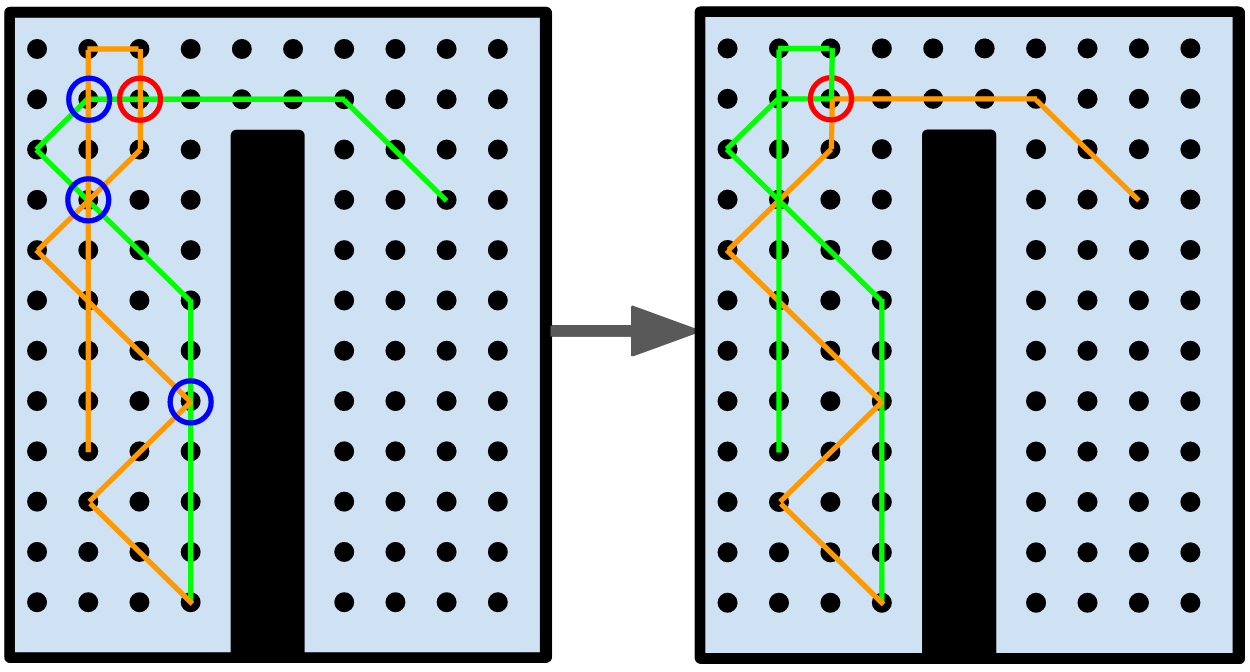
\includegraphics[width=0.8\linewidth]{figures/crossover.png}
\caption{An example of the crossover mechanism. First, common waypoints are found (marked in blue and red). Next, one of the common waypoints is chosen at random (red). Finally, the tails of the two paths are swapped, as shown on the right.}
\label{fig:crossover}
\end{figure}

\subsubsection{Mutation}

After a new chromosome is generated, either by cloning or crossover, it is subjected to two different types of mutation ($\mathcal{A}$ and $\mathcal{B}$), each with a defined probability of occurring. The first type of mutation ($\mathcal{A}$) randomly selects both a random gene in the chromosome and a random length between the current and maximum chromosome length. Using the traversable graph, a new path is randomly generated from that gene onward, up to the randomly chosen length. See Fig. \ref{fig:mutation} for an example of this style of mutation.

\begin{figure}
\centering
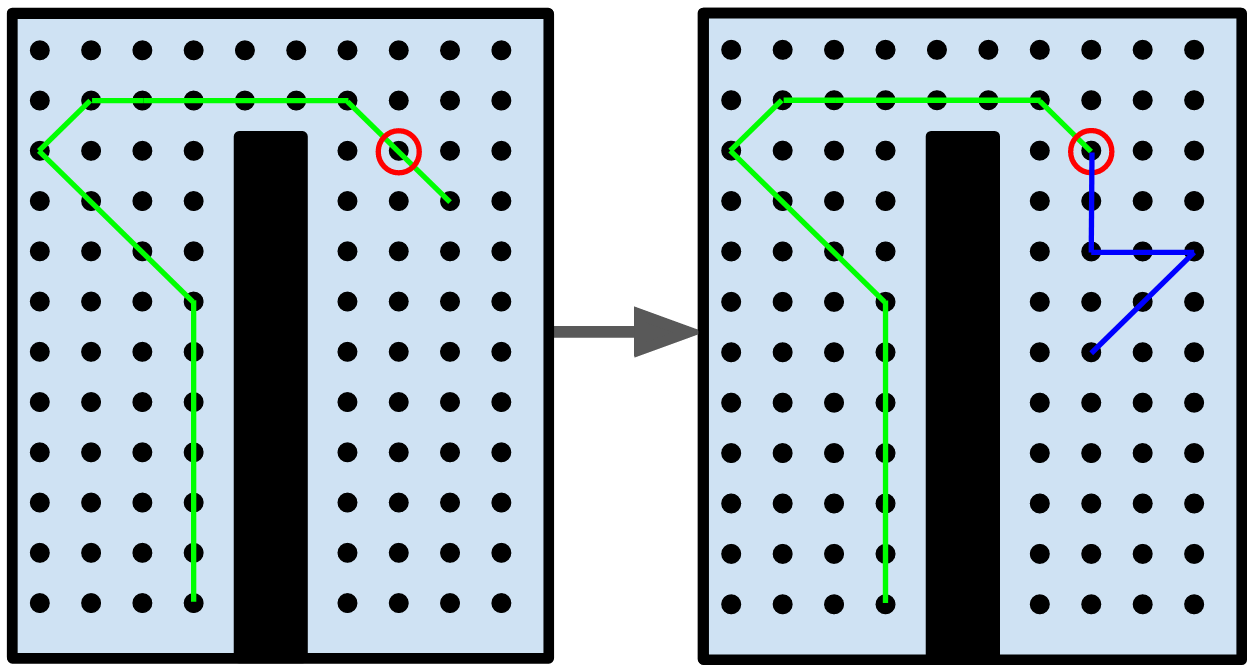
\includegraphics[width=0.8\linewidth]{figures/mutation.png}
\caption{An example of the Mutation $\mathcal{A}$ mechanism. A random waypoint in the path is chosen (marked in red) and the tail is replaced with a random path of a random length.}
\label{fig:mutation}
\end{figure}

The second mutation ($\mathcal{B}$) is intended to straighten and shorten the paths. A random segment (random in position, static in length) of the chromosome is selected. The hamming distance from the first waypoint in the segment to all other waypoints in the segment, starting with the last point, is computed. If a point is found to be within two waypoints of the first point in the segment, all waypoints in the segment between those two are replaced with a shortcut, as illustrated in Fig. \ref{fig:muterpolation}. This is only completed according to a defined sub-probability of mutation, which is typically much higher than the overall mutation probability. The segment is left as is if no points are within a hamming distance of two. This type of mutation is applied to the chromosome a specified number of times with the intent of finding multiple useful shortcuts in the path.

\begin{figure}
\centering
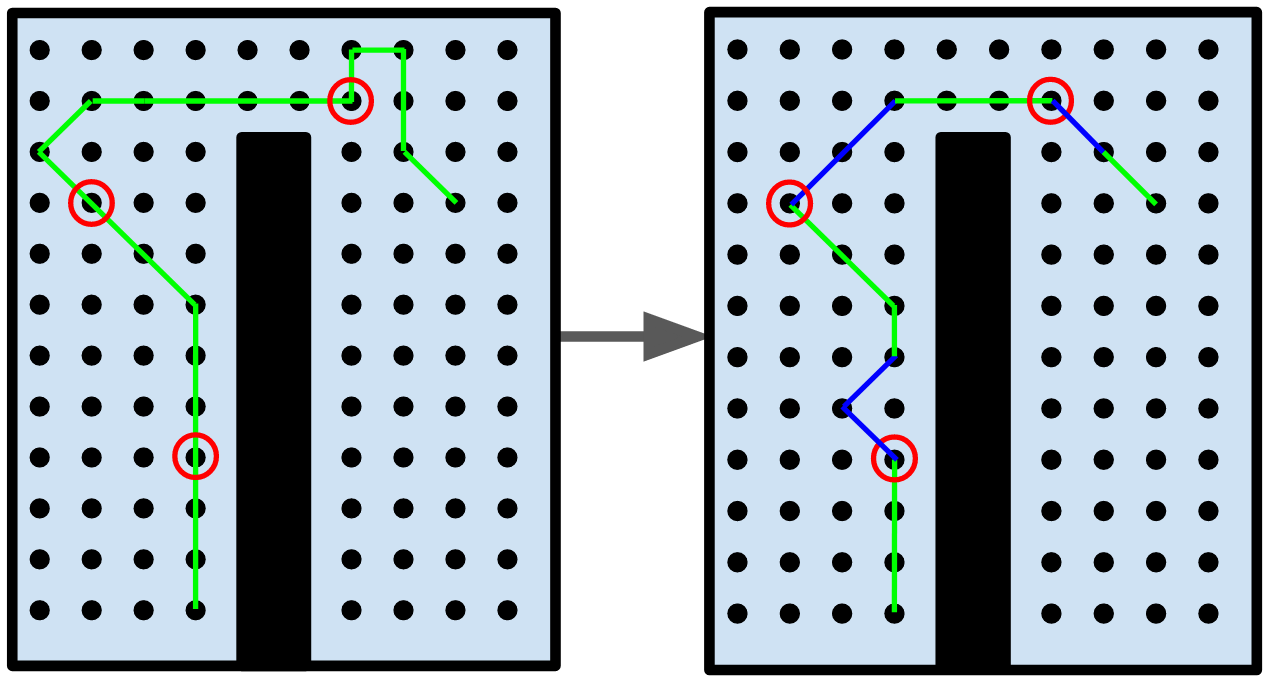
\includegraphics[width=0.8\linewidth]{figures/muterpolation.png}
\caption{An example of the Mutation $\mathcal{B}$ mechanism. Multiple random points are chosen (marked in red). From each point, the path is searched up to a certain length to find places where shortcuts or alternate paths can be taken (shown as blue segments).}
\label{fig:muterpolation}
\end{figure}

\subsubsection{Constraints}\label{constraints}

Most of the constraints of the system are modeled into the discretization, traversability graph, and upper and lower bounds of the chromosome length as described in Section \ref{setup}. However, constraining the minimum coverage and loop closures could not be applied directly to the model.

The coverage constraint was applied by adding to the cost to make it worse than the worst feasible design. Since we are using two objectives we implemented this constraint by adding a large cost to the flight time objective to guarantee that all organisms violating the constraint will be dominated by other designs (according to the maximin fitness).

Rather than start with a high constraint that would eliminate many of the original designs, we initialized the constraint with a low value. Over several generations we increase the constraint slowly to push the designs into the desired region of objective space. This also inadvertently increases the average flight time, but as the system continues to evolve, more efficient flight paths are found even with the new, strict coverage constraint and the average flight time decreases again.

We defined loop closures as anywhere that the path passes through the same waypoints in the same direction more than once as shown in Fig. \ref{fig:loop_closure}. For a path to satisfy the loop closure constraint, it has to have a set number of loop closures. To avoid useless loop closures, a loop closure is only counted towards the constraint if it is separated by at least a defined number of waypoints. Similarly to the coverage constraint, we enforce this constraint by adding a large cost to the coverage, ensuring that all paths that violate the constraint are dominated by other designs.

\begin{figure}
\centering
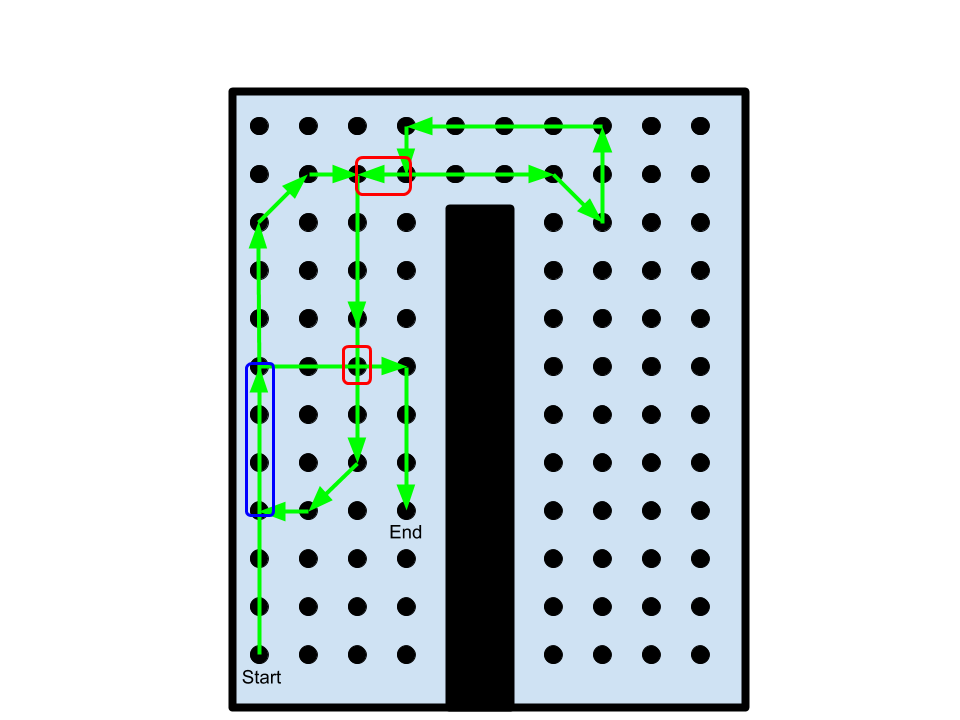
\includegraphics[width=1.0\linewidth]{figures/loop_closure.png}
\todo{change colors or something, this is hard to see}
\caption{An example of single agent loop closure. A valid loop closure is marked in blue where the path passes through the same waypoints in the same direction. Examples of times when the path crosses over its self but not loop closures are marked in red.}
\label{fig:loop_closure}
\end{figure}

As described in \cite{Parkinson2019}, constraints are applied to the fitness value. Because we have two objectives, and our non-modeled constraints directly relate to only one of the objectives, we implement these constraints on the objective values prior to computing the fitness value for the organism.

\subsubsection{Maximin and Elitism}

After all of a generation's children have been created, the fitness of the parents and children is computed by using the maximin fitness function as described by Balling \cite{Balling2003}. In brief, the maximin scheme encourages a spread of designs across the Pareto front between competing objective values, with a target of minimizing the objectives. It does this by calculating the distance between each of the objective values of all the organisms, and finds the minimum difference of both objectives to each other. It then computes the maximum of all of these minima as the fitness value. Following the notation in \cite{Parkinson2019}, if $f_k^i$ is the computed $k^{\mathrm{th}}$ objective value for organism $i$, the maximin fitness for organism $i$ is computed by,

\begin{equation}%\nonumber
    fitness = \max_{i \neq j}\left(\min_{k}\left(f_k^i - f_k^j\right)\right).
\end{equation}

Once all parents and children have fitness values computed with respect to each other, the best $N$, comprising of the most negative fitness values, is selected as the next generation, where $N$ is the size of a generation.

\subsubsection{Low-Variance Sampling}

We use a Roulette-style sampling method to pick parents in a way that gives organisms with better designs (determined by the maximin fitness) a higher probability of being selected as a parent for the crossover process. We employ a low-variance sampling technique as described in \cite{Thrun2006}. This method normalizes the population's fitnesses and treats them as a set of probabilities. A naive approach randomly samples $N$ times from the pool of parents according to their respective probabilities. In order to reduce the possibility of a parent being sampled disproportionately to its probability, we draw a single uniform random number $r$ between 0 and $\tfrac{1}{N}$. The probabilities are then stacked up and compared to $r$. Whichever organism corresponds to the bin that $r$ falls into gets sampled and $\tfrac{1}{N}$ is added to $r$ and again compared to the stack of probabilities. This process is repeated $N$ times. We also apply fitness pressure with the low variance sampling with a tunable parameter $\gamma$ with a value between 0 and 1. If $\gamma$ = 0, no fitness pressure is applied, and the sample is random. If $\gamma$ = 1, it will only select the most fit organism for the next generation.

%%%%%%%%%%%%%%%%%%%%%%%%%%%%%%%%%%%%%%%%%%%%%%%%%%%%%%%%%%%%%%%%%%%%%%%%%%%%%%%%
\subsection{Multi-Agent Architecture}

The following section details the changes and addittions to the architecture to generate multi-agent paths.

\subsubsection{Chromosome}
The chromosome was expanded to be of size $nxl_{max}$ where $n$ is the number of agents and $l_{max}$ is the maximum path length where each row represents the path of its respective agent. The genes each row have the same representation as in the single agent case. To accommodate for paths that are shorter than the maximum length, any path shorter than $l_max$ is padded with -1 at the end to populate any unused genes in the chromosome. We also allow for the agents to either start at the same waypoint as each other (if there were only one entry to the map), or different waypoints (if there are different entrances into the map).

\subsubsection{Crossover}
Crossover is largely the same as the single agent case. It treats each agent separately and preforms crossover on each path independantly.

\subsubsection{Mutation}
Much like crossover, the mutation mechanisms were only modified to accept the new chromosome structure. We treat each agent separately as mutation $\mathcal{A}$ and $\mathcal{B}$ are performed on the chromosome.

\subsubsection{Constraints}
The majority of the architecture change was in modeling the constraints for the multi-agent case. The constraint on coverage was applied to the combined coverage of the full chromosome, not the individual paths. The loop closure constraint had to be expanded to handle loop closures between agents. In order for a single 3D map to be generated when dealing with more than one agent, the agents must have loop closures between each other. For only two or three agents, this is still simple to enforce. After four agents, graph theory is necessary to efficiently evaluate the connectivity of the paths.

To keep track of loop closures, we create a symmetric $nxn$ loop closure matrix $C$ with each element defined by

\begin{align}
  c_{ij} &= \text{loop closures between agent } i \text{ and agent } j \\
  i,j &= 0...n \nonumber
\end{align}

where $n$ is the number of agents. The values along the diagonal of $C$ are the number of loop closures the agent has with its own path. The off-diagonal terms store the total number of loop closures between agent $i$ and agent $j$. The loop closure constraint from the single agent architecture is applied here using these values to ensure that paths loop close with themselves. We also added a new constraint to ensure the agents paths are connected enough to build a single map.

As described by \cite{Weisstein}, we create the $nxn$ symmetric adjacency matrix $A$ from the loop closure matrix $C$ with each element defined by

\begin{align}
  a_{ij} &=
  \begin{cases}
    1, & \text{if } (c_{ij} \geq 1 \text{ and } i \neq j)\\
    0, & \text{otherwise}
  \end{cases}\\
  i,j &=0 ...n \nonumber
\end{align}

which encodes which agents are directly connected to other agents
Then we create the $nxn$ diagonal degree matrix $D$ defined by

\begin{align}
  d_{ii} &= \sum_{j=0}^{n} a_{ij} \\
  i &= 0 ... n \nonumber
\end{align}

So each element along the diagonal represents the number of agents that agent is directly connected to through loop closure. Next, we define the Graph Laplacian Matrix $L$ as

\begin{equation}
  L = D-A
\end{equation}

which encodes the connectivity of the agents. We can determine whether there are enough loop closures between agents to connect all paths into a single map by looking at the eigenvalues of $L$. The number of zero eigenvalues represents the number of separate connected components in the graph. So if all agents are connected to each other, there will be only one zero eigenvalue. If there are not sufficient loop closures to combine into a single map, there will be more than one zero eigenvalue. We use this to set the last constraint used for the multi-agent architecture. There must be exactly one zero eigenvalue of $L$ to satisfy the constraint. An example connectivity graph for a system with five agents is shown in Fig. \ref{fig:connectivity}

\begin{figure}
\centering
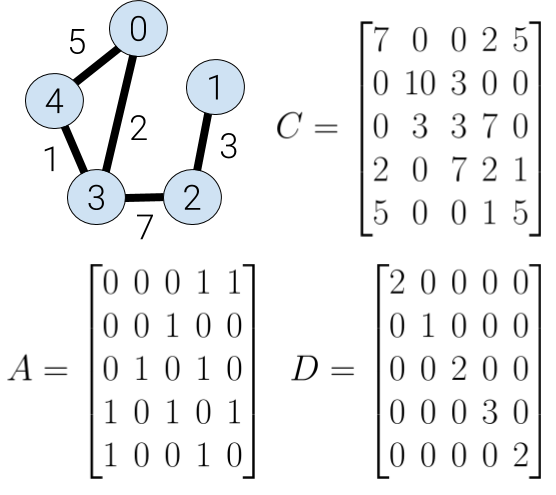
\includegraphics[width=0.8\linewidth]{figures/connectivity.png}
\caption{An example connectivity graph with five agents and its respective loop closure matrix $C$, adjacency matrix $A$, and degree matrix $D$. The agent number is labeled on each blue node and the number of loop closures between agents is shown with the black edges between nodes.
%C=\begin{bmatrix}
 %7 &  0 &  0 & 2 & 5\\
 %0 &  10&  3 & 0 & 0\\
 %0 &  3 &  3 & 7 & 0\\
 %2 &  0 &  7 & 2 & 1\\
 %5 &  0 &  0 & 1 & 5
%\end{bmatrix}
%A=\begin{bmatrix}
% 0 &  0 &  0 & 1 & 1\\
% 0 &  0 &  1 & 0 & 0\\
% 0 &  1 &  0 & 1 & 0\\
% 1 &  0 &  1 & 0 & 1\\
% 1 &  0 &  0 & 1 & 0
%\end{bmatrix}
% D=\begin{bmatrix}
 % 2 &  0 &  0 & 0 & 0\\
 % 0 &  1 &  0 & 0 & 0\\
 % 0 &  0 &  2 & 0 & 0\\
 % 0 &  0 &  0 & 3 & 0\\
 % 0 &  0 &  0 & 0 & 2
% \end{bmatrix}
}
\label{fig:connectivity}
\end{figure}


\subsubsection{Maximin and Elitism}
The maximin fitness function is the same as with a single agent except that the coverage value used is the total negative coverage of all the agents summed together and the scaled total flight time of all the agents are used as the objective values. Elitism remains the same.

\subsubsection{Low-Variance Sampling}
The low variance sampling did not need modification for the multi-agent architecture.

%%%%%%%%%%%%%%%%%%%%%%%%%%%%%%%%%%%%%%%%%%%%%%%%%%%%%%%%%%%%%%%%%%%%%%%%%%%%%%%%
\section{RESULTS}\label{results}
\todo{this section needs to be updated to show new results single agent with loop closures and multi-agent}
The designer is required to set many parameters for the genetic algorithm to work as derived in \cite{Parkinson2019}. The parameters we used, along with parameters specific to our implementation, are outlined in Table \ref{tab:parameters}.

\begin{table}
  \caption{Parameters used to obtain described results}
\begin{tabular}{l|l}
\hline
\multicolumn{1}{|l|}{Parameter}                 & \multicolumn{1}{l|}{Value} \\ \hline
Generation Size (Organisms)                        & 100                     \\
Crossover Probability                              & 0.7                     \\
Crossover Time Threshold (Waypoints)               & 70                      \\
Mutation $\mathcal{A}$ Probability                 & 0.3                     \\
Mutation $\mathcal{B}$ Probability                 & 0.3                     \\
Number of Mutation $\mathcal{B}$ Instances         & 20                      \\
Mutation $\mathcal{B}$ Acceptance Probability      & 0.8                     \\
Mutation $\mathcal{B}$ Search Distance (Waypoints) & 5                       \\
Objective Scaling Factor : Flight Time             & 0.0001                  \\
Objective Scaling Factor : Coverage                & -1.0                    \\
Coverage Blending Factor $\alpha_{cov}$            & 1.0                     \\
Coverage Sections                                  & 15                      \\
Minimum Chromosome Length (Waypoints)              & 75                      \\
Maximum Chromosome Length (Waypoints)              & 250                     \\
Pixel Scale (meters/pixel)                         & 0.15                    \\
Minimum Coverage Constraint Start                  & 0.3                     \\
Minimum Coverage Constraint End                    & 0.8                     \\
Minimum Coverage Constraint Aging (Generations)    & 60                      \\
Loop Closure Separation Threshold (Waypoints)      & 30                      \\
Minimum Loop Closures                              & 2                       \\
Path Memory (Waypoints)                            & 10                      \\

\todo{update this table to show all variables symbols}\\
\end{tabular}
\label{tab:parameters}
\end{table}

\subsection{Single Agent}
\subsubsection{Fitness}

\begin{figure*}
\centering
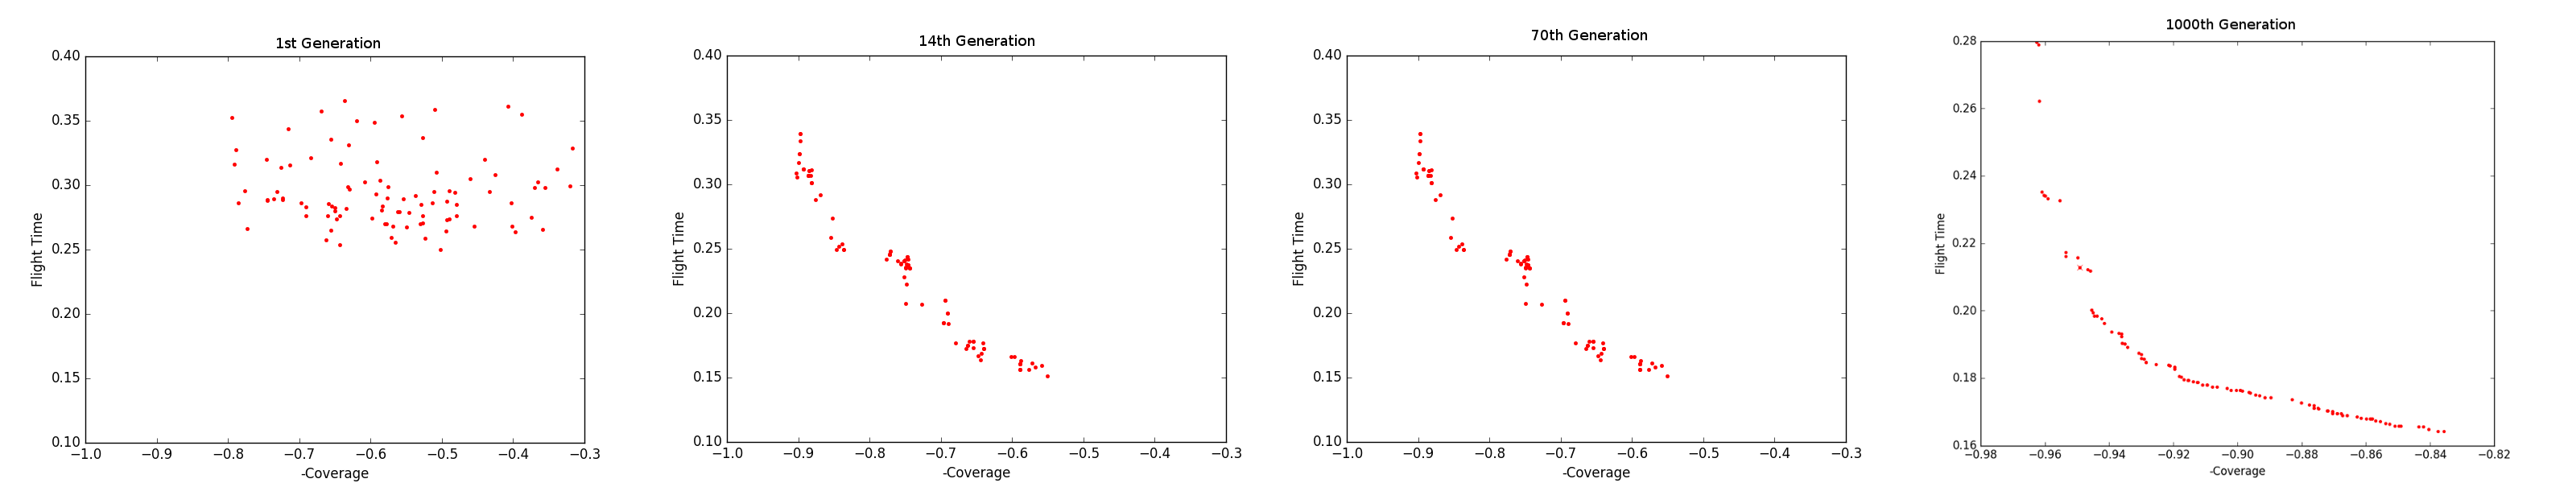
\includegraphics[width=1.0\linewidth]{figures/pareto_history2.png}
\todo{make this bigger so it is more useful}
\caption{History of the Pareto front across several generations. The dynamic constraint placed on coverage prioritizes high coverage but also induces high flight time for the first 100 generations. Afterward, the algorithm can work with high coverage organisms, optimizing them for lower flight times, while maintaining their high coverage properties.}
\label{fig:pareto_cheetos}
\end{figure*}

\begin{figure*}
\centering
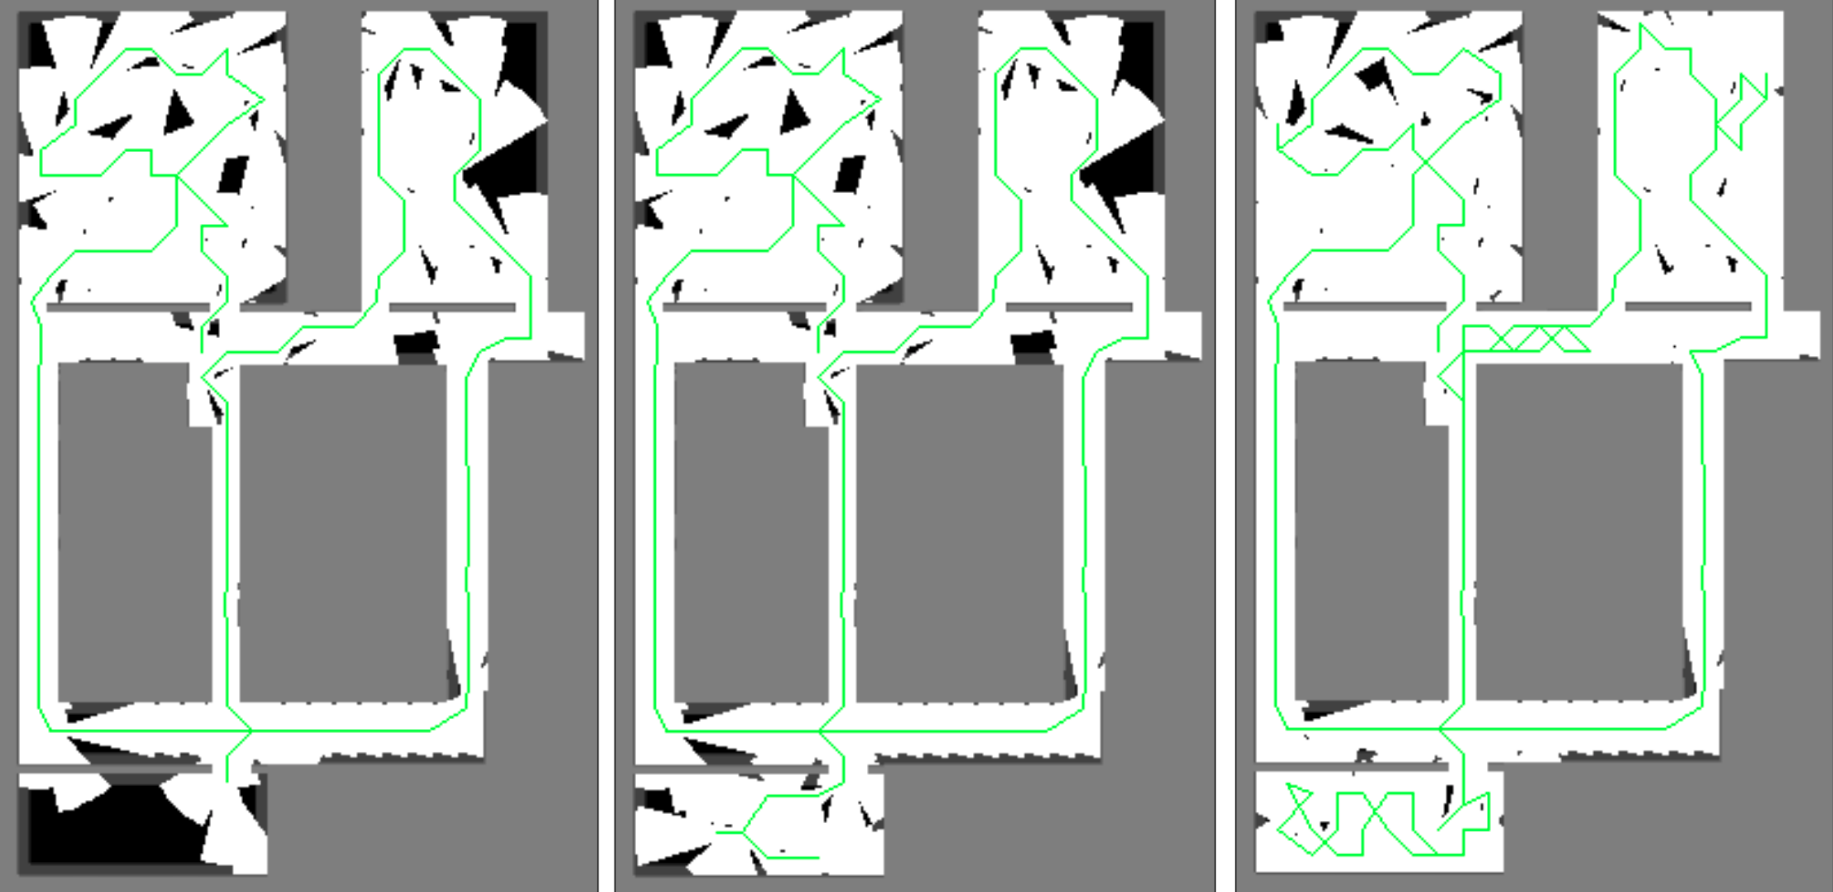
\includegraphics[width=1.0\linewidth]{figures/final_paths.png}
\caption{Examples of final paths generated by the genetic algorithm. These paths show example paths from the extremes of the Pareto front that display shortest flight time with less coverage (left), and best coverage with higher flight time (right). The center shows a good path from the middle of the Pareto front, with a good balance of flight time and coverage.}
\label{fig:final_paths}

\end{figure*}

Fig. \ref{fig:pareto_cheetos} shows how the objective values of the organisms evolved from generation to generation. Four different snapshots are shown: the first, randomly generated set of parents, the state of the generation at about a third and two-thirds of the way through the selected number of generations, and last, the final result of the progression of 1000 generations. Fig. \ref{fig:objectives} shows how the average negative coverage and average flight time progresses over the course of the 600 generations. The coverage flattens out temporarily, but then continues to drop after 400 generations. The interesting result displayed is in the flight time objective value history. After about 30 generations, the flight time starts to rise again. This is due to the dynamic constraint that invalidates all organisms with coverage below the defined threshold at the defined generation number. Once the coverage constraint settles to a constant value, the organisms with good coverage dominate the generation population and the algorithm successfully lowers the flight time again to represent a useful Pareto front that has a good spread of options from which to choose.

\begin{figure}
\centering
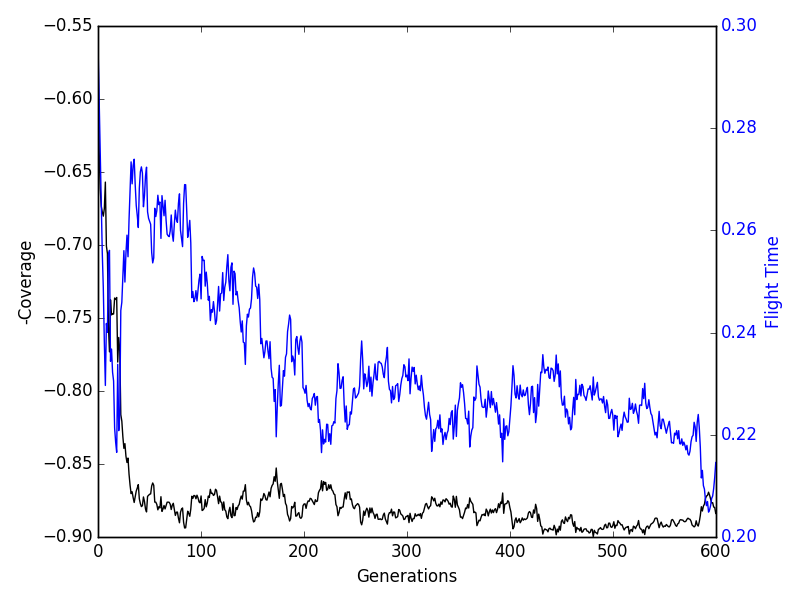
\includegraphics[width=0.8\linewidth]{figures/fitness.png}
\caption{A plot of the average objective values over 600 generations. Note how the average flight time initially decreases then sharply increases again, as the rolling constraint on coverage is applied. As the generations are then allowed to evolve, the flight time settles back down below the previous minimum.}
\label{fig:objectives}
\end{figure}

\subsubsection{Paths Generated}

Our algorithm was successful in generating useful paths, as seen in Fig. \ref{fig:final_paths}. The path on the left shows the option with the shortest flight time. However, it misses an entire room at the bottom left of the 2D map. Via our crossover and mutation schemes, the good elements that cause this path to have a short flight time, such as straighter paths with minimal overlap, are able to propagate to other path designs. The path on the right shows excellent coverage close to 100\%, but it also includes too much overlap with itself, wasting the drone battery supply. The path in the center of the figure shows how the maximin fitness and our implementation of the genetic algorithm were able to produce a design with the good elements from both. The path in the center includes coverage in the lower left room with minimal waste of the battery supply looping back over places already visited.


\subsection{Multiple Agents}
\subsubsection{Fitness}
\subsubsection{Paths Generated}
%%%%%%%%%%%%%%%%%%%%%%%%%%%%%%%%%%%%%%%%%%%%%%%%%%%%%%%%%%%%%%%%%%%%%%%%%%%%%%%%
\section{CONCLUSIONS}\label{conclusions}

We were able to successfully generate paths with reasonably good coverage that do not appear to meander too much for a single UAV. Future work on this project will include adding loop closure detection into the model to significantly increase the quality of generated 3D maps. We also plan to extend this to work with multiple UAVs flying simultaneously. We expect the need to use the paths generated with a lower level path planner that can dynamically change waypoints according to obstacles and other unmapped disparities. Finally we plan to test the paths generated both in high fidelity simulation as well as in hardware.

%%%%%%%%%%%%%%%%%%%%%%%%%%%%%%%%%%%%%%%%%%%%%%%%%%%%%%%%%%%%%%%%%%%%%%%%%%%%%%%%

\bibliographystyle{IEEEtran} % We choose the "plain" reference style
\bibliography{genetic_coverage_paper_2019}

\end{document}
